\documentclass[11pt]{article}

\usepackage{amssymb, amsmath, mathtools, color, fontspec, bm}
\usepackage{ifxetex, ifluatex, microtype}

\setsansfont{Roboto}
\setmainfont{Roboto}

\usepackage[affil-it]{authblk}

\PassOptionsToPackage{hyphens}{url} % url is loaded by hyperref

\usepackage[unicode=true]{hyperref}

\PassOptionsToPackage{usenames, dvipsnames}{color} % color is loaded by hyperref

\hypersetup{
            pdftitle={A lineage-based Markov tree model to quantify cellular heterogeneity},
            pdfkeywords={cancer, heterogeneity, lineage, hidden Markov Model},
            pdfborder={0 0 0},
            breaklinks=true}
\urlstyle{same}  % don't use monospace font for urls

\usepackage[margin=1in, letterpaper]{geometry}

\usepackage[]{biblatex}
\addbibresource{./manuscript/references.bib}


\usepackage{longtable,booktabs}
\usepackage{graphicx,grffile}
\makeatletter
\def\maxwidth{\ifdim\Gin@nat@width>\linewidth\linewidth\else\Gin@nat@width\fi}
\def\maxheight{\ifdim\Gin@nat@height>\textheight\textheight\else\Gin@nat@height\fi}
\makeatother
% Scale images if necessary, so that they will not overflow the page
% margins by default, and it is still possible to overwrite the defaults
% using explicit options in \includegraphics[width, height, ...]{}
\setkeys{Gin}{width=\maxwidth,height=\maxheight,keepaspectratio}
\IfFileExists{parskip.sty}{%
\usepackage{parskip}
}{% else
\setlength{\parindent}{0pt}
\setlength{\parskip}{6pt plus 2pt minus 1pt}
}
\setlength{\emergencystretch}{3em}  % prevent overfull lines
\providecommand{\tightlist}{%
  \setlength{\itemsep}{0pt}\setlength{\parskip}{0pt}}
\setcounter{secnumdepth}{0}
% Redefines (sub)paragraphs to behave more like sections
\ifx\paragraph\undefined\else
\let\oldparagraph\paragraph
\renewcommand{\paragraph}[1]{\oldparagraph{#1}\mbox{}}
\fi
\ifx\subparagraph\undefined\else
\let\oldsubparagraph\subparagraph
\renewcommand{\subparagraph}[1]{\oldsubparagraph{#1}\mbox{}}
\fi

% set default figure placement to htbp
\makeatletter
\def\fps@figure{htbp}
\makeatother

% Defines absolute value paired delimiter "\abs{}"
\DeclarePairedDelimiter\abs{\lvert}{\rvert}

\title{A lineage-based Markov tree model to quantify cellular heterogeneity}

\author[a]{Spongebob Squarepants}
\author[a]{Patrick Star}
\author[a]{Squidward Tentacles}
\author[a]{Gary}
\author[a]{Mr.~Krabs}
\author[a,b]{Aaron S. Meyer}

\affil[a]{Department of Bioengineering, Jonsson Comprehensive Cancer Center, Eli
and Edythe Broad Center of Regenerative Medicine and Stem Cell Research;
University of California, Los Angeles}
\affil[b]{Contact info}

\date{}

\newcommand{\beginsupplement}{\cleardoublepage%
      \setcounter{table}{0}
      \renewcommand{\thetable}{S\arabic{table}}%
      \setcounter{figure}{0}
      \renewcommand{\thefigure}{S\arabic{figure}}%
}

\begin{document}
\maketitle


\begin{abstract}
Chemotherapy is one of the primary methods of cancer treatment due to
its ability to impede the growth of highly prolific cancer cells. One of
the main obstacles to successful chemotherapy treatment is that highly
prolific cancer cells naturally display non-uniform responses to
therapy. It therefore becomes imperative for oncologists to prescribe
chemotherapy combinations which target all subpopulations of cells in a
given patient's tumor. Classifying the heterogeneous resistance of
cancer cells may potentially enable the design of therapies that are
tumor-specific and thus enable all malignant cells within a tumor to
respond adequately and die. Current methods of intratumor cell
classification possess low specificity because they use population-level
measurements, such as IC50, to gauge cellular responses to cancer
therapy. In addition, these methods rely on single timepoint
measurements which mask cancer cell evolution dynamics. In this paper,
we present a novel computational method that utilizes cell lineage trees
to learn the characteristic patterns of cell heterogeneity de novo and
predict variable response to drug in tumors over time. TODO METHODS.
TODO RESULTS. TODO DISCUSSION.
\end{abstract}


\hypertarget{summary-points}{%
\section{Summary points}\label{summary-points}}

\begin{itemize}
\tightlist
\item
  One
\item
  Two
\item
  Three
\end{itemize}

\hypertarget{author-summary}{%
\section{Author Summary}\label{author-summary}}

Cell heterogeneity, such as variability in drug response, arises as
cells proliferate. \emph{Shared} heterogeneous traits, such as a
response to drug like resistance or susceptibility within a
subpopulation, are correlated across a lineage because resistant
subpopulations most likely diverged from a common progenitor or a set of
common progenitors that were \emph{also} resistant or had acquired
traits leading to resistance. These acquired traits of resistance may be
the result of responses to cellular microenvironments, epigenetics,
and/or mutations. Using lineage tree information, we hope to capture
these dynamic transitions between heterogeneous latent states of cells
and arrive with a more accurate identification of cell heterogeneity in
a tumor. Our computational approach employing Markov random field theory
provides higher specificity through identifying intratumor resistance on
an individual cell level based on lineage histories and enables
real-time identification of changes in resistance throughout therapy.

\hypertarget{introduction}{%
\section{Introduction}\label{introduction}}

In 2018, over 1.7 million new cases of cancer were estimated to be
diagnosed with over 609,000 of those cases projected to be
fatal.\textsuperscript{\protect\hyperlink{ref-SmithCancerScreening}{1}}
Most primary treatments of cancer consists of chemotherapy
(i.e.~cytotoxic and endocrine therapies), whereby patients are given
chemicals that destroy highly-prolific cells to stall cancer growth or
eliminate the tumor. However, the ability of therapy to impede tumor
growth varies significantly due to the vast heterogeneity in intratumor
response to
therapy.\textsuperscript{\protect\hyperlink{ref-LungHeterogeneity}{2},\protect\hyperlink{ref-ColorectalHeterogeneity}{3}}
Specifically, each tumor consists of cancer cell subpopulations that
differ in terms of cell intrinsic and extrinsic factors including
genetic plasticity, epigenetic alterations, and micro-environmental
stressors.\textsuperscript{\protect\hyperlink{ref-BreastMicroEnv}{4}--\protect\hyperlink{ref-HistoneInhibi}{7}}
Complete cancer remission is predicated on delivering therapies that
eliminate all malignant cancer subpopulations within a tumor. Current
drug-screening protocols involve giving known cancer cell lines
different drug doses and evaluating therapy performance based on the
percent of cells killed and the dose required to have a half-maximal
effect.\textsuperscript{\protect\hyperlink{ref-chauvin2017high}{8},\protect\hyperlink{ref-QuantitativeHistology}{9}}
However, these metrics for therapy performance solely provide en bloc
averages of overall tumor response to therapy that fail to consider the
vast complexity of subpopulation heterogeneity. In addition, the
significant proportion of cells acquiring resistance at a time point
stochastically after subjection to therapy must be identified with a
novel, real-time analytic
method.\textsuperscript{\protect\hyperlink{ref-GenotypicEGFR}{10}--\protect\hyperlink{ref-clonalMutationalEvolution}{12}}

Intratumor heterogeneity causes distinct differences in cell phenotype
among cancer cells. The cell transformations originate from underlying
cell-intrinsic factors, such as genomic alterations (i.e.~altered
nucleotide excision repair and telomere maintenance), and cell-extrinsic
factors such as spatial variability in vasculature and environmental
stressors causing DNA promoter
mutations.\textsuperscript{\protect\hyperlink{ref-BreastMicroEnv}{4}--\protect\hyperlink{ref-HistoneInhibi}{7},\protect\hyperlink{ref-TNBpatterns}{13}}
Cancer cell plasticity, which is difficult to predict, further
exacerbates the heterogeneity problem, as two daughter cells of the same
non-resistant parent cell have been seen in extreme cases to acquire
substantial therapy
resistance.\textsuperscript{\protect\hyperlink{ref-Stochasticstatetransitions}{14}}
The clinical implication of cell-to-cell heterogeneity is intratumor
variability in therapy resistance that leads to poor outcomes and low
remission, as primary tumors that relapse after treatment possess
significantly more subpopulation diversity than relapse-free
tumors.\textsuperscript{\protect\hyperlink{ref-Cancerstemcells}{15}}

\hypertarget{materials-and-methods}{%
\section{Materials and Methods}\label{materials-and-methods}}

\hypertarget{cell-culture-experiments}{%
\subsection{Cell Culture Experiments}\label{cell-culture-experiments}}

\hypertarget{cell-culture-set-up}{%
\subsubsection{Cell Culture Set-up}\label{cell-culture-set-up}}

To model a heterogeneous tumor, we conducted a proof-of-concept
experiment by co-culturing cells derived from lung adenocarcinoma: PC-9
and H1299. These cells were obtained from the Meyer Lab at UCLA, where
PC-9 cells were already transfected to fluoresce red through a H2B
(histone h2b)-mKate2 nuclear localization lentivirus (Sigma-Aldrich,
St.~Louis, MO) and H1299 green through a H2B-GFP lentivirus
(Sigma-Aldrich, St.~Louis, MO). Before co-culturing, PC-9 and H1299
cells were grown separately in monolayers in tissue culture-treated well
plates, using complete media (Roswell Park Memorial Institute media with
L-glutamine (Thermo Fisher Scientific, Canoga Park, CA), supplemented
with 5\% fetal bovine serum (Corning, Corning, NY) and 1\%
penicillin/streptomycin (Thermo Fisher Scientific, Canoga Park, CA)).
Similar conditions for the well plates and media were used for the
co-culture experiment. Cells were passaged every 3 days and thrown out
after 9 passages. Co-Culture Set-up and Imaging To co-culture PC-9 and
H1299 cells, 200 PC-9 cells/cm2 and 200 H1299 cells/cm2 were taken from
their respective well plates and seeded in complete media. Once seeded,
cells were treated with 100 nM erlotinib (Selleckchem, Houston, TX), an
epidermal growth factor receptor inhibitor which causes significant
growth inhibition in PC-9 cells (IC50 = 7 nM) but not in H1299 cells
(IC50 \textgreater{} 10 μM).Cells were incubated in the Incucyte S3
Live-Cell Analysis System (Incucyte, Ann Arbor, MI) and imaged using
phase contrast and fluorescent microscopy. The green channel excitation
and emission ranges were 440-480 nm and 504-544 nm, respectively,
whereas the red channel excitation and emission ranges were 565-605 nm
and 625-705 nm, respectively. The exposure times were 300 ms for the
green channel and 400 ms for the red channel. A 20x objective with a
numerical aperture of 0.45 was used. Imaging started 24 hours after
initial seeding to allow cells to adhere, and images were acquired every
5 minutes for 4 days.

\hypertarget{cell-tracking-and-lineage-generation}{%
\subsubsection{Cell Tracking and Lineage
Generation}\label{cell-tracking-and-lineage-generation}}

To generate lineage trees from the acquired images, a cell image
analysis software, ilastik (European Molecular Biology Laboratory,
Heidelberg, Germany), was used to track the cells from the time-lapse
datasets. Before inputting the imagesets into ilastik, Fiji's ImageJ
(NIH) Stackreg plugin was used to correct for in-plane drift. Moving to
ilastik, pixel classification was used to segment the images, and we
employed a tracking with deep learning workflow to training the program
on true cell divisions and false detections. This allowed us to
construct lineage tracks and link objects between frames. Upon running
the pipeline to completion, the output was exported as a comma-separated
values (CSV) file containing identification numbers for each cell and
corresponding parent cells for each image. Using this CSV file, the
parameters of interest, such as cell fate, longevity, and cell type were
extracted using the Python programming language.

\hypertarget{single-state-model}{%
\subsection{Single state model}\label{single-state-model}}

We first build a model of cell growth based on the phenotypic
measurement of cells. The first measurement is the cell's fate, encoded
as \(\phi\) ,where \(\phi\in\{0,1\}\), a binary event where \(\phi=0\)
is the cell dying at the end of its lifetime, and \(\phi=1\) is the cell
dividing into two daughter cells. The second measurement is the cell's
lifetime, encoded as \(\tau\), where \(\tau\in (0, +\infty)\), a
positive real number indicating how long the cell lived in hours. For
example, a complete observation could be of the form
\(\bm{x}_{m} = (1, 20)\) where cell \(m\) divided into two daughter
cells after living for 20 hours. In general, for any observation
\(\bm{x}_{n}\) for cell \(n\), we have a tuple indicating the cell fate
and the cell lifetime, \(\bm{x}_{n}=(\phi_{n}, \tau_{n})\). To
probabilistically model each observation, the cell fate follows a
Bernoulli distribution with Bernoulli rate parameter \(p_{B}\) where
\(p_{B}\in[0,1]\) and \(p_{B}\) represents the probability of
\(\phi=1\), the chance that a cell divides. The cell lifetime follows a
noninformatively-censored Exponential distribution with Exponential rate
parameter \(\beta_{E}\). The Exponential distribution models the
mortality of cells over time. These underlying parameters also describe
the states in the multiple state model discussed later.TODO

\hypertarget{multiple-state-model}{%
\subsection{Multiple state model}\label{multiple-state-model}}

\hypertarget{model-description}{%
\subsubsection{Model description}\label{model-description}}

Using the parent-daughter links each cell has, we can construct lineage
trees which then capture information about the history of cells in the
context of their families. Furthermore, for each observation
\(\bm{x}_{n}\) corresponding to cell \(n\) in our lineage tree, we
introduce a latent or hidden variable \(\bm{z}_{n}\) which takes one of
\(K\) discrete values, \(\bm{z}_{n}\in\{1,2,\ldots,K\}\). Ultimately,
our proposed tHMM is comprised of two trees, an observed probabilistic
tree and a hidden probabilistic tree. The observed probabilistic tree is
defined by the set of hierarchal nodes
\(\bm{X}=\left\lbrace\bm{x}_{1},\bm{x}_{2},\ldots,\bm{x}_{N}\right\rbrace\)
where \(N\) is the number of total cells or observations in our lineage
tree. Furthermore, we have a similar construction of the hidden
probabilistic tree, defined by the set of hierarchal nodes
\(\bm{Z}=\left\lbrace\bm{z}_{1},\bm{z}_{2},\ldots,\bm{z}_{N}\right\rbrace\).
The hidden probabilistic tree and the observed probabilistic tree have
the same indexing structure. It is important to note that the cell at
node \(n\) is not necessarily the parent of the cell at node \(n+1\) and
that the the cell at node \(n\) is not necessarily the daughter of the
cell at node \(n-1\). However, because it is important to denote such
relationships not only when describing lineage trees, but also when
describing the relevant probability distributions, we introduce
\(\bm{P}(n)\) to denote the cell that is the parent of the cell at node
\(n\), and \(\bm{C}(n)\) to denote the set of children of the cell at
node \(n\). Furthermore, the cell at node \(n=1\) or the root node will
always be the initial cell in the lineage tree, or the root cell. Cells
at the end of the lineage tree, that is to say, cells at the leaves of
the tree (nodes with only one edge or only one adjacent node) will be
denoted by the set \(\bm{L}\). All other cells (cells at nodes that are
not leaves) will be denoted by the set \(\bm{nL}\).

To fully describe both trees, we say that a joint distribution
\({P}(\bm{Z},\bm{X})\) follows the tree hidden Markov property if and
only if
\[{{P}(\bm{Z},\bm{X}) = P}(\bm{z}_{1},\bm{z}_{2},\ldots,\bm{z}_{N},\bm{x}_{1},\bm{x}_{2},\ldots,\bm{x}_{N}) = {P}(\bm{z}_{1})\prod_{n=2}^{N}{P}(\bm{z}_{n}\mid\bm{z}_{\bm{P}(n)})\prod_{n=1}^{N}{P}(\bm{x}_{n}\mid\bm{z}_{n})\]
This factorization of the joint distribution follows from the
conditional independence properties of our emissions (i.e.~observations)
and the Markov tree dependence of the latent variables. These can be
easily derived form the Bayesian network diagram in \textbf{Figure 3}
which graphically shows the influence of each variable on the other. The
similarity to the factorization of hidden Markov chains (HMCs) is also
evident, the main difference being that the transition probabilities for
tHMMs are \({P}(\bm{z}_{n}\mid\bm{z}_{\bm{P}(n)})\) and the transition
probabilities for HMCs are \({P}(\bm{z}_{n}\mid\bm{z}_{(n-1)})\).

\hypertarget{parameters}{%
\subsubsection{Parameters}\label{parameters}}

Each factor in the tree hidden Markov property in represents a key
parameter in the tHMM. Fully describing it with known values specifies
the entire model. The following parameters are similar to those used in
describing HMCs.

We first introduce the hyperparameter \(K\) which is the number of
possible discrete hidden states the hidden variables can take. This is
the only parameter the user is required to input as all the other
parameters depend on the value of \(K\). Ultimately, each state
\(k\in\{1,2,\ldots,K\}\) uniquely describes the distributions (Bernoulli
and Exponential distributions) via the respective parameters
(\(p_{B}^{(k)}\) and \(\beta_{E}^{(k)}\)) governing the respective
observations or emissions (cell fate \(\phi\) and cell lifetime
\(\tau\)) for a group of cells. By ascribing a group of cells in the
lineage tree a particular state \(k\in\{1,2,\ldots,K\}\), we can
identify subpopulations of interest based on the ascribed states of
other groups of cells. For example, if the root cell was found to be of
state \(1\), that is to say, \(\bm{z}_{1}=1\), but all cells at the
leaves further down in the lineage were found to be of state \(2\), then
it is reasonable to assume that sometime in the lineage, a transition
between states \(1\) and \(2\) occurred. One can then further
interrogate and ascribe meaning to each of the states. That is, if state
\(1\) described a Bernoulli distribution with Bernoulli rate parameter
\(p_{B}^{(1)}=0.5\) but state \(2\) described a Bernoulli distribution
with Bernoulli rate parameter \(p_{B}^{(2)}=0.9\), then state \(2\) can
be identified as cells that are resilient or highly proliferative
compared to cells of state \(1\). The meaning ascribed to each state is
furnished by the user upon interrogation of the distributions that each
state uniquely describes. Sometimes the number of states \(K\) can be
arbitrarily chosen; for example, if the number of states selected equals
the number of cells totally observed, that is, \(K=N\), then each cell
will be ascribed its own unique state and the goal of using our model to
identify heterogeneity is trivialized. To prevent an arbitrary selection
of \(K\), the Akaike information criterion (AIC) is used for model
selection and can inform the user of what value of \(K\) is best.

Once the number of discrete states \(K\) is chosen, the three other
parameters describing tree hidden Markov property can be built. The
first parameter is a vector of initial hidden state priors or an initial
probability distribution over the set of states. This describes the
probability \(P(\bm{z}_{1})\), or more explicitly, \(P(\bm{z}_{1}=k)\)
for some state \(k\in\{1,2,\ldots,K\}\), which is then encoded as
\(\pi_{k}\). That is to say, \(\pi_{k}\) is the probability that the
hidden root node is of state \(k\) for \(k\in\{1,2,\ldots,K\}\). Note
that for some states \(j\in\{1,2,\ldots,K\}\), \(\pi_{j}=0\), implying
that they cannot be initial states. This is stored as a
\(K\)-dimensional vector \(\bm{\pi}\) where the \(j\)-th entry is
\(\pi_{j}=P(\bm{z}_{1}=j)\) for \(j\in\{1,2,\ldots,K\}\).

The second parameter is a matrix of state transition probabilities
stored as a square \(K\times K\) matrix \(\bm{T}\). Each element of the
matrix \(T_{jk}\) represents the probability of going to state \(k\)
(column-element) from state \(j\) (row-element). More explicitly,
\(T_{jk} = {P}(\bm{z}_{n}=k\mid\bm{z}_{\bm{P}(n)}=j)\) for some states
\(j,k \in \{1,2,\ldots,K\}\). Note that the diagonal of \(\bm{T}\)
consists of entries of the form \(T_{kk}\), the probability of the child
state inheriting same state as the parent cell.

The third parameter is \(K\)-long dictionary of parameters for the
distributions each state uniquely describes. We call this dictionary
\(\bm{E}=\{E_{1},E_{2},\ldots,E_{K}\}\) where for some
\(k\in\{1,2,\ldots,K\}\), the parameters describing the distributions of
state \(k\) are stored as \(E_{k}=\{p_{B}^{(k)},\beta_{E}^{(k)}\}\).
This parameter describes the final remaining factor in the tree hidden
Markov property, the emission likelihoods
\({P}(\bm{x}_{n}\mid\bm{z}_{n})\). More explicitly, for some state
\(k\in\{1,2,\ldots,K\}\) and for some observation
\((\phi_{n}, \tau_{n})\), we are trying to describe the probability
\({P}(\bm{x}_{n}=(\phi_{n}, \tau_{n})\mid\bm{z}_{n}=k)\). Here we assume
the observations are conditionally independent given then respective
state variable or we assume a Naive Bayes condition on the emissions
(each feature or observation \(\phi_{n},\tau_{n}\) is conditionally
independent of the other given the category or state \(k\)):

\hypertarget{acknowledgements}{%
\section{Acknowledgements}\label{acknowledgements}}

This work was supported by NIH DP5-OD019815 to A.S.M. \textbf{Competing
financial interests:} The authors declare no competing financial
interests.

\hypertarget{author-contributions-statement}{%
\section{Author contributions
statement}\label{author-contributions-statement}}

A.S.M. conceived of the study.

\beginsupplement

\hypertarget{supplement}{%
\section{Supplement}\label{supplement}}

\begin{figure}
\hypertarget{fig:supp1}{%
\centering
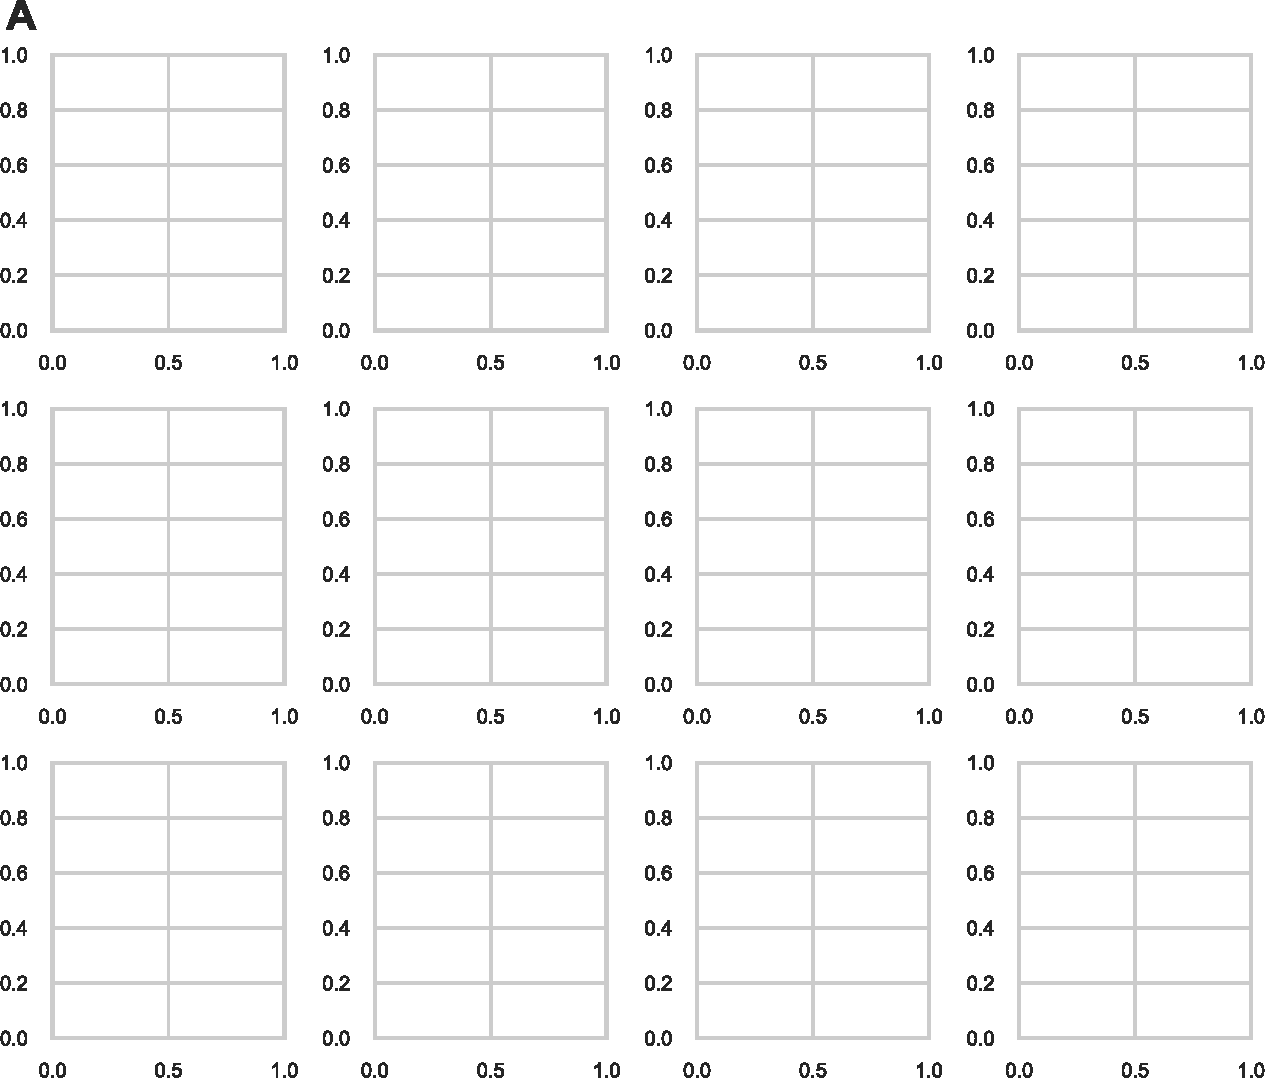
\includegraphics{./figures/figureS1.pdf}
\caption{\textbf{Title of supplement 1.} XXX}\label{fig:supp1}
}
\end{figure}

\begin{figure}
\hypertarget{fig:supp2}{%
\centering
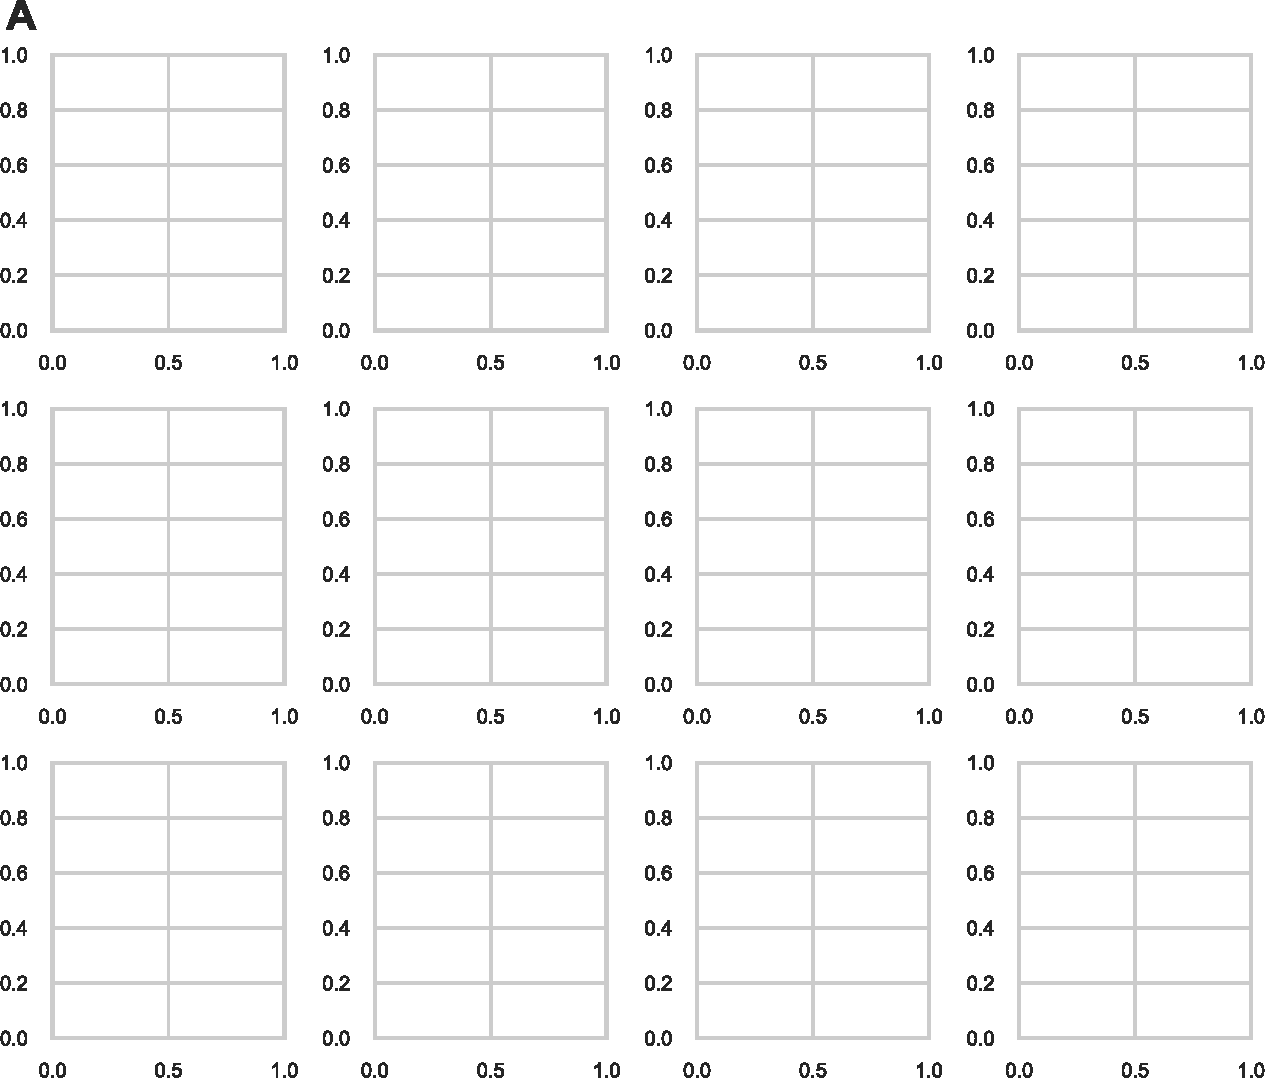
\includegraphics{./figures/figureS2.pdf}
\caption{\textbf{Title of supplement 2.} XXX}\label{fig:supp2}
}
\end{figure}

\begin{figure}
\hypertarget{fig:supp3}{%
\centering
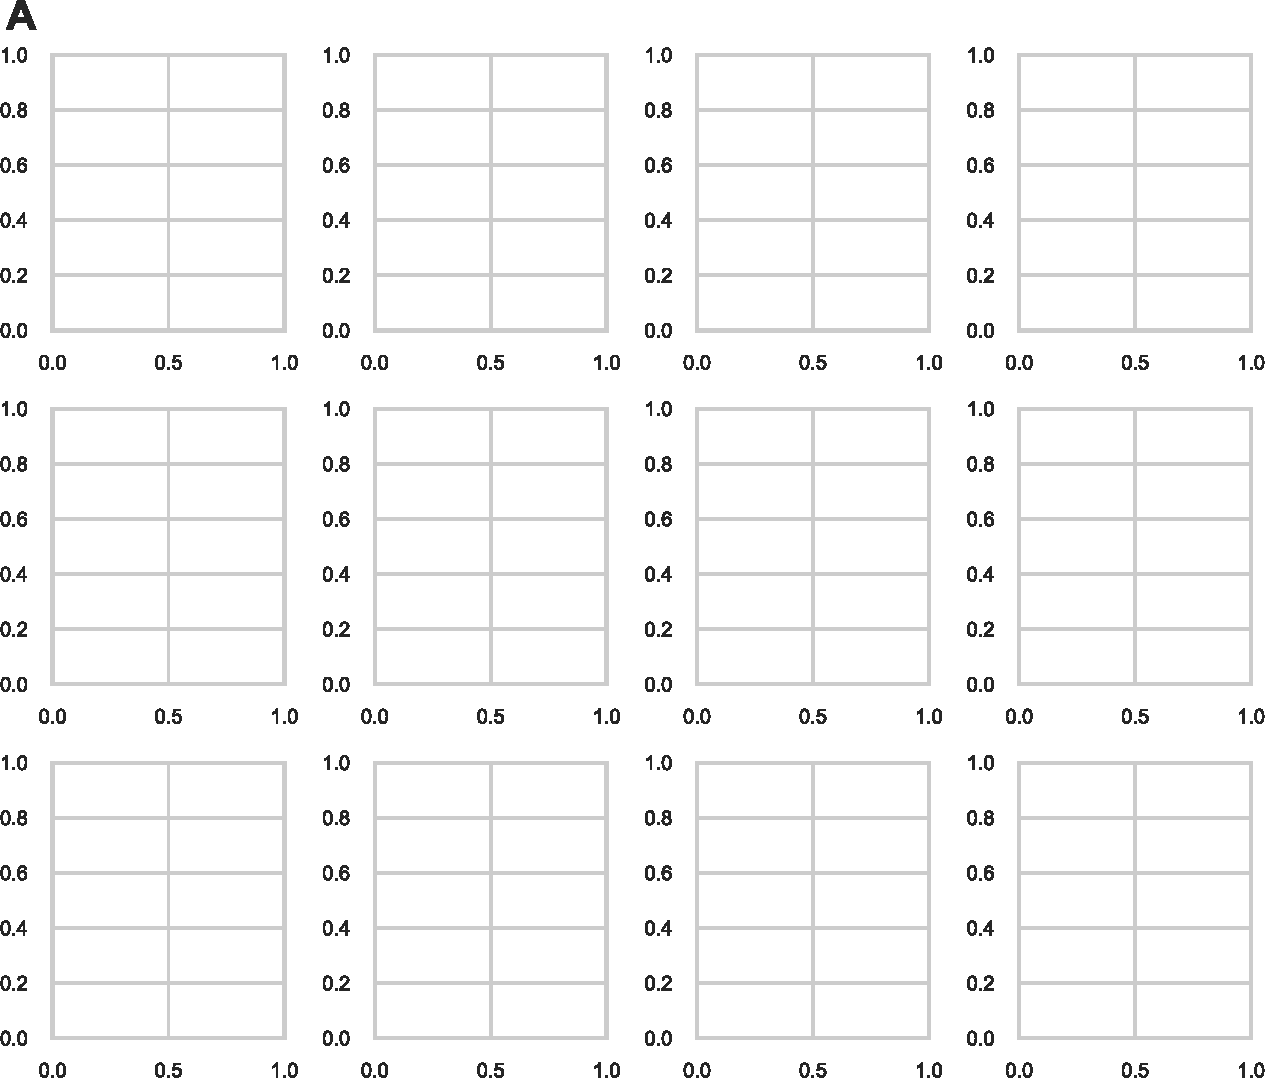
\includegraphics{./figures/figureS3.pdf}
\caption{\textbf{Title of supplement 3.} XXX}\label{fig:supp3}
}
\end{figure}

\begin{figure}
\hypertarget{fig:supp4}{%
\centering
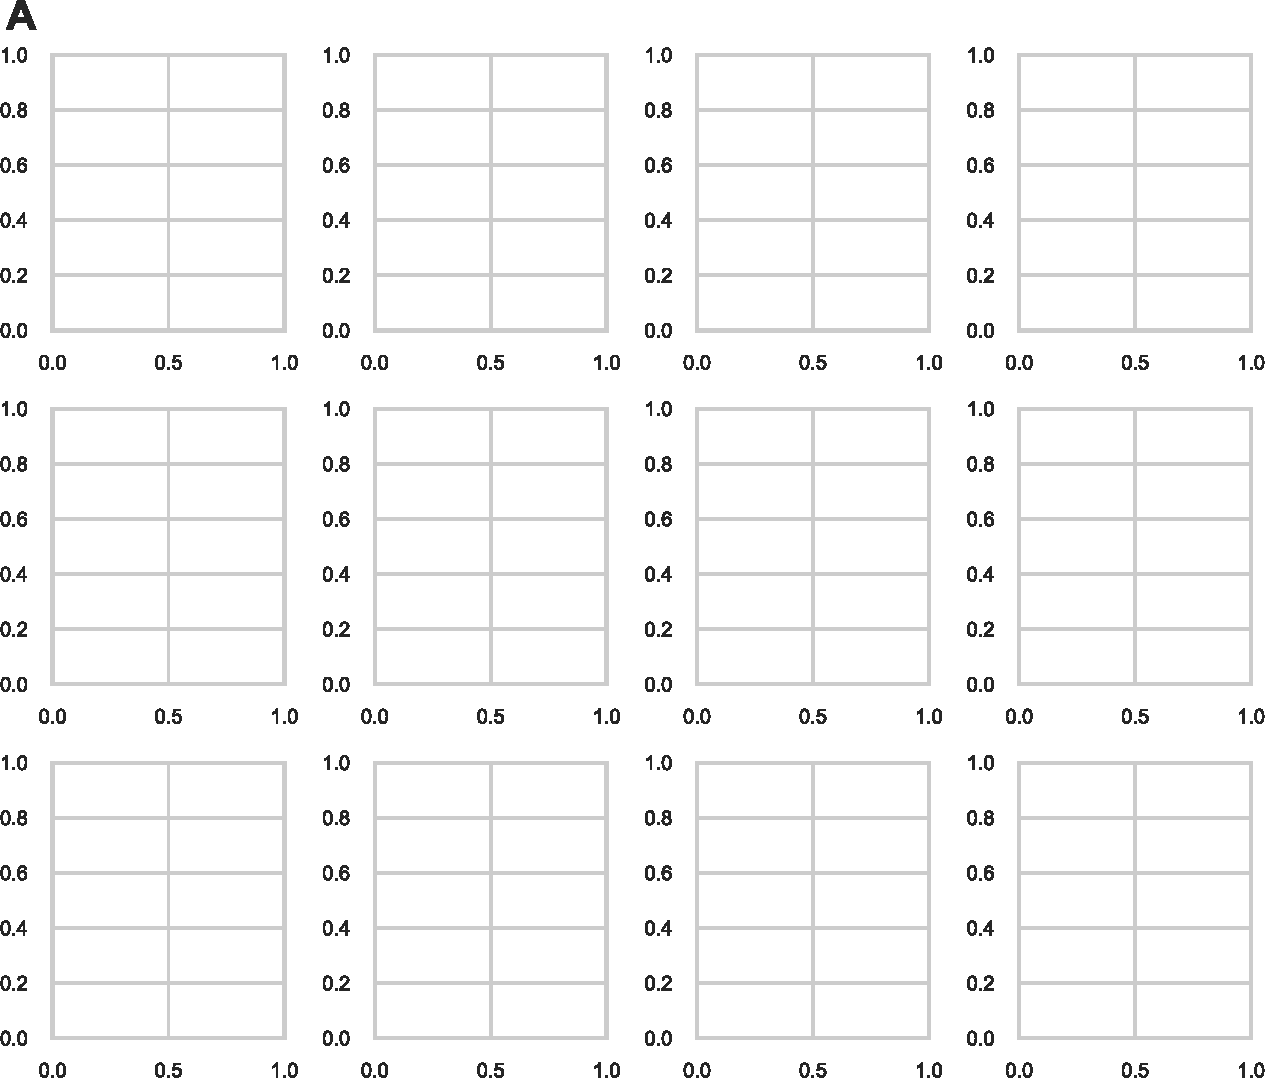
\includegraphics{./figures/figureS4.pdf}
\caption{\textbf{Title of supplement 4.} XXX}\label{fig:supp4}
}
\end{figure}

\begin{figure}
\hypertarget{fig:supp5}{%
\centering
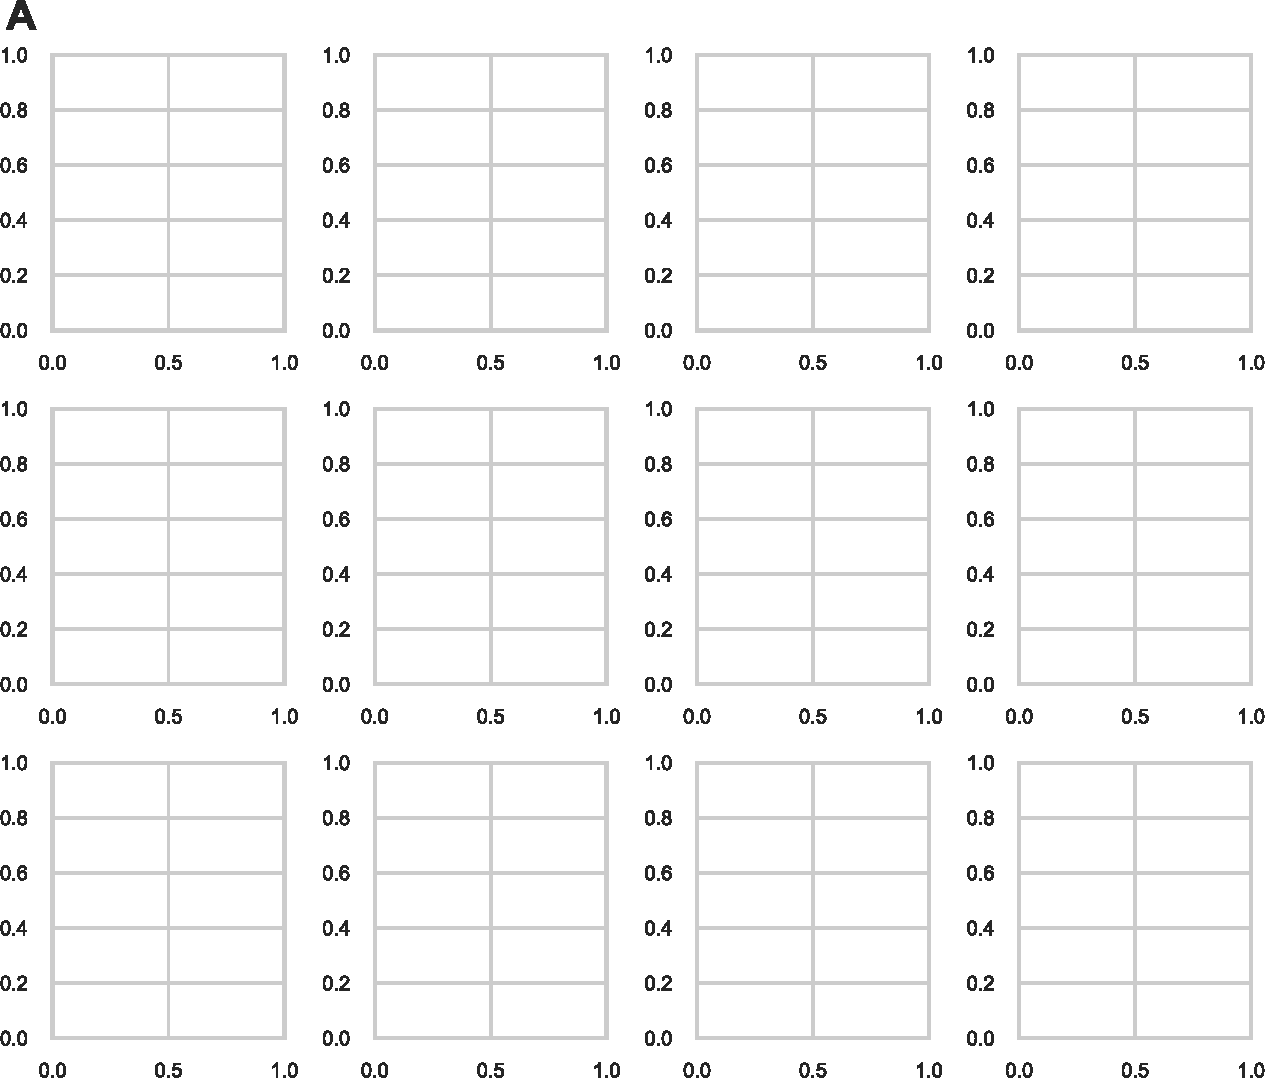
\includegraphics{./figures/figureS5.pdf}
\caption{\textbf{Title of supplement 5.} XXX}\label{fig:supp5}
}
\end{figure}

\cleardoublepage

\hypertarget{references}{%
\section*{References}\label{references}}
\addcontentsline{toc}{section}{References}

\hypertarget{refs}{}
\leavevmode\hypertarget{ref-SmithCancerScreening}{}%
1. Smith, R. A. Cancer screening in the united states, 2018: A review of
current american cancer society guidelines and current issues in cancer
screening. \emph{CA: A Cancer Journal for Clinicians} \textbf{68,}
297--316 (2018).

\leavevmode\hypertarget{ref-LungHeterogeneity}{}%
2. Di Maio, M. \emph{et al.} Chemotherapy-induced neutropenia and
treatment efficacy in advanced non-small-cell lung cancer: A pooled
analysis of three randomised trials. \emph{The lancet oncology}
\textbf{6,} 669--677 (2005).

\leavevmode\hypertarget{ref-ColorectalHeterogeneity}{}%
3. De Roock, W. \emph{et al.} Effects of kras, braf, nras, and pik3ca
mutations on the efficacy of cetuximab plus chemotherapy in
chemotherapy-refractory metastatic colorectal cancer: A retrospective
consortium analysis. \emph{The lancet oncology} \textbf{11,} 753--762
(2010).

\leavevmode\hypertarget{ref-BreastMicroEnv}{}%
4. Semenza, G. L. The hypoxic tumor microenvironment: A driving force
for breast cancer progression. \emph{Biochimica et Biophysica Acta
(BBA)-Molecular Cell Research} \textbf{1863,} 382--391 (2016).

\leavevmode\hypertarget{ref-Chemokines}{}%
5. Nagarsheth, N., Wicha, M. S. \& Zou, W. Chemokines in the cancer
microenvironment and their relevance in cancer immunotherapy.
\emph{Nature Reviews Immunology} \textbf{17,} 559 (2017).

\leavevmode\hypertarget{ref-EpigeneticMod}{}%
6. Feinberg, A. P., Koldobskiy, M. A. \& Göndör, A. Epigenetic
modulators, modifiers and mediators in cancer aetiology and progression.
\emph{Nature Reviews Genetics} \textbf{17,} 284 (2016).

\leavevmode\hypertarget{ref-HistoneInhibi}{}%
7. Falkenberg, K. J. \& Johnstone, R. W. Histone deacetylases and their
inhibitors in cancer, neurological diseases and immune disorders.
\emph{Nature Reviews Drug discovery} \textbf{13,} 673 (2014).

\leavevmode\hypertarget{ref-chauvin2017high}{}%
8. Chauvin, C. \emph{et al.} High-throughput drug screening identifies
pazopanib and clofilium tosylate as promising treatments for malignant
rhabdoid tumors. \emph{Cell reports} \textbf{21,} 1737--1745 (2017).

\leavevmode\hypertarget{ref-QuantitativeHistology}{}%
9. Lan, C. \emph{et al.} Quantitative histology analysis of the ovarian
tumour microenvironment. \emph{Scientific reports} \textbf{5,} 16317
(2015).

\leavevmode\hypertarget{ref-GenotypicEGFR}{}%
10. Sequist, L. V. \emph{et al.} Genotypic and histological evolution of
lung cancers acquiring resistance to egfr inhibitors. \emph{Science
translational medicine} \textbf{3,} 75ra26--75ra26 (2011).

\leavevmode\hypertarget{ref-CGANComprehensiveMolecular}{}%
11. Network, C. G. A. \& others. Comprehensive molecular portraits of
human breast tumours. \emph{Nature} \textbf{490,} 61 (2012).

\leavevmode\hypertarget{ref-clonalMutationalEvolution}{}%
12. Shah, S. P. \emph{et al.} The clonal and mutational evolution
spectrum of primary triple-negative breast cancers. \emph{Nature}
\textbf{486,} 395 (2012).

\leavevmode\hypertarget{ref-TNBpatterns}{}%
13. Dent, R. \emph{et al.} Triple-negative breast cancer: Clinical
features and patterns of recurrence. \emph{Clinical cancer research}
\textbf{13,} 4429--4434 (2007).

\leavevmode\hypertarget{ref-Stochasticstatetransitions}{}%
14. Gupta, P. B. \emph{et al.} Stochastic state transitions give rise to
phenotypic equilibrium in populations of cancer cells. \emph{Cell}
\textbf{146,} 633--644 (2011).

\leavevmode\hypertarget{ref-Cancerstemcells}{}%
15. Enderling, H. Cancer stem cells: Small subpopulation or evolving
fraction? \emph{Integrative Biology} \textbf{7,} 14--23 (2014).

\printbibliography

\end{document}
